As has been discussed in the previous sections, we are interested in visualizing
and understanding the difference in performance between predictive and
horizontal auto-scaling for two different pod initialization times and two
different traffic patterns. As such, we have two different tests on which we
compare ERU and QoS: increase-decrease traffic pattern with 135s pod
initialization time and flash-crowd traffic pattern with 135s pod initialization time.

For each test on the matrix, we provide two different sources of information.
First, we generate a graph comparing the summation of ERU and QoS across the 40
minute evaluation time for predictive and reactive auto-scaling. Additionally,
we provide statistical measurements for the difference of predictive and
reactive auto-scaling at the same point in the evaluation sequence (i.e. we
compare the summation of ERU and QoS after 10 minutes for predictive with the
summation of ERU and QoS after 10 minutes for reactive). With respect to
statistical measurements, we calculate a one-sided p-value
based on the null hypothesis that the difference
between the summation of ERU and QoS for predictive and reactive auto-scaling is
$0$. As we are interested in seeing if predictive auto-scaling performs better
than reactive auto-scaling, we calculate a one-sided p-value, $p$, with the alternative
hypothesis that the difference between the summation of ERU and QoS for
predictive and reactive auto-scaling is greater than $0$. We test for
significance at the $5\%$ significance level, meaning that if $p < 0.05$, we can
reject our null hypothesis in favor of our alternative hypothesis that
predictive auto-scaling performs better than reactive auto-scaling for this
combination of traffic pattern and pod initialization time.

\subsubsection{135s and increase-decrease}

\begin{figure}[!h]
  \centerline{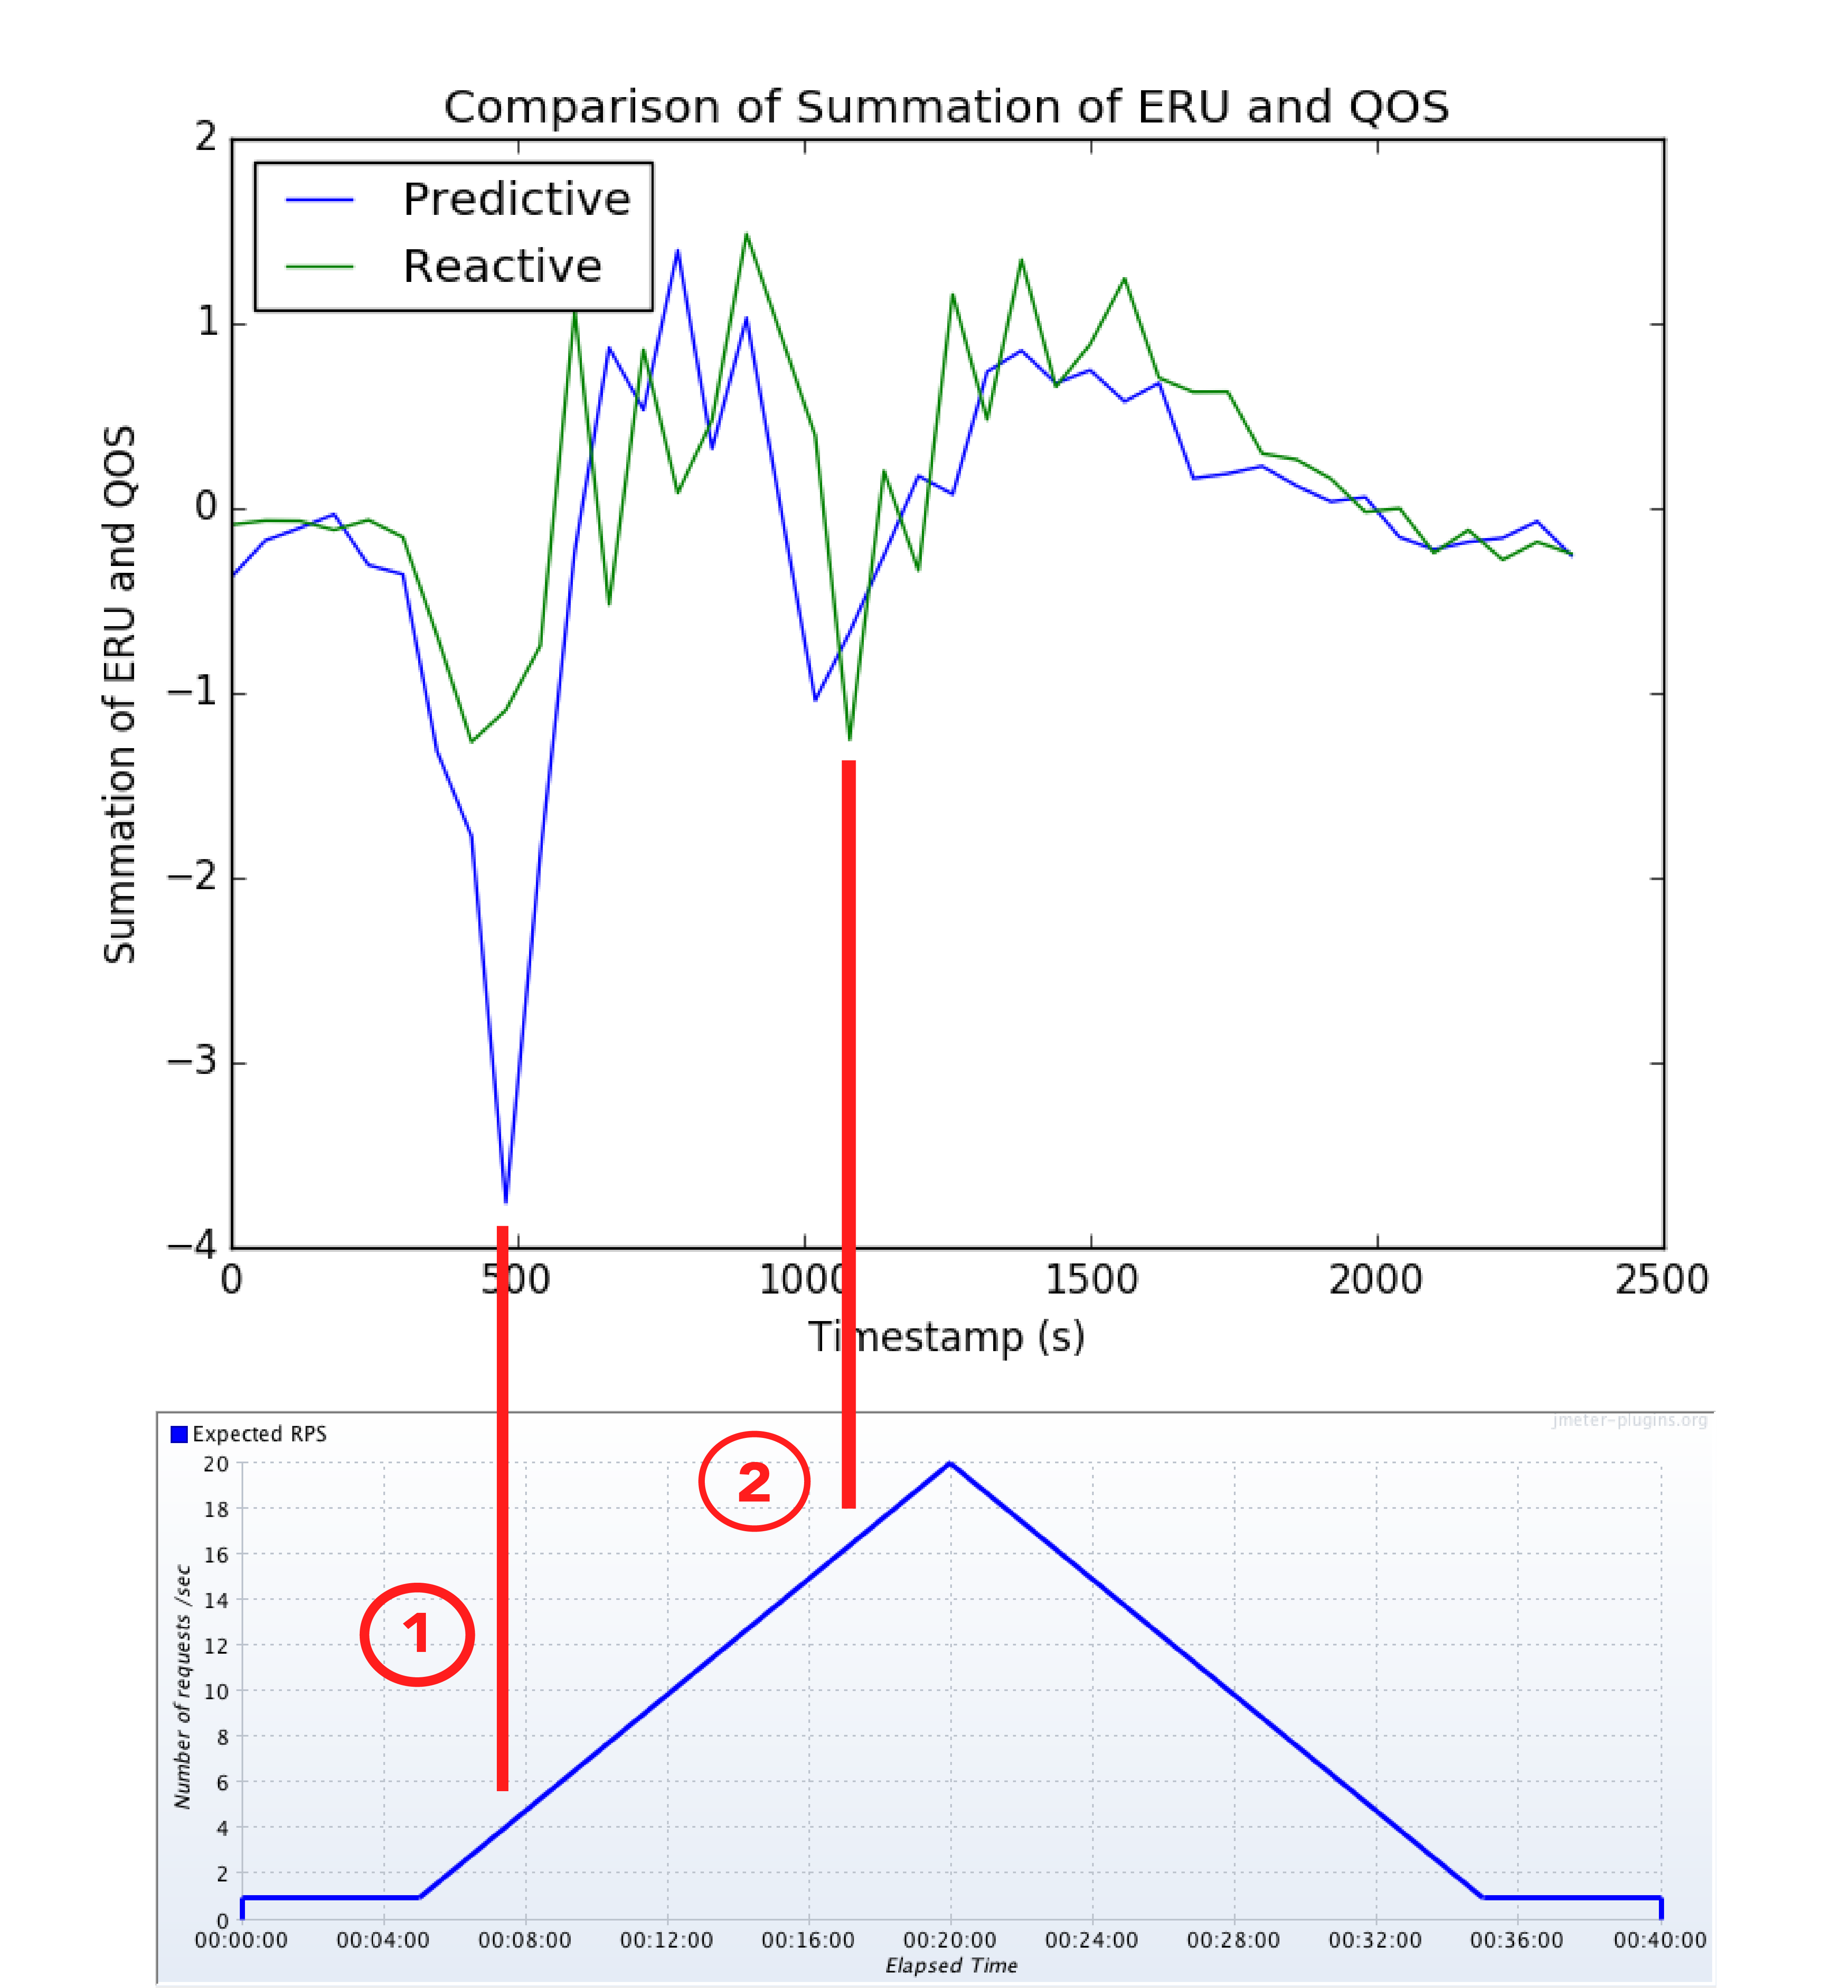
\includegraphics[scale=.70]{increase-decrease-labelled.png}}
  \caption{A comparison of the summation of ERU and QoS for
    predictive and reactive auto-scaling for 135s, increase-decrease.}
  \label{fig:135s-increase-decrease-labelled}
\end{figure}

Figure \ref{fig:135s-increase-decrease-labelled} contains a graph
showing predictive and reactive auto-scaling's different
summations of efficient resource utilization and quality of service over the
course of the \textit{increase-decrease} trial. In contrast to our previous two
traffic patterns, we find that predictive auto-scaling is not particularly
beneficial in this context. Specifically, if we look at the moment labelled
$1$ on Figure \ref{fig:135s-increase-decrease-labelled}, we an instance in which
predictive auto-scaling suffers a severe performance decrease in comparison to
reactive auto-scaling. We trace this decrease again to under-provisioning. In
this scenario, the introductory buffer period has caused our linear prediction
algorithm to underestimate the slope of the line indicating the rise in load. As
such, the reactive auto-scaling algorithm actually has a more aggressive opinion
of the load the application will face. As this aggressive understanding is
confirmed by our actual increase, reactive auto-scaling outperforms predictive
auto-scaling on the \textit{increase-decrease} traffic-pattern. Scenario
$1$ is in contrast to the scenario labelled $2$, in which predictive
auto-scaling performs equally to reactive auto-scaling, because it is no longer
negatively impacted by previous measurements which do not reflect the current
slope.

\begin{table}[htbp]
  \centering
  \caption{Difference in Predictive and Reactive Auto-scaling for 135s,
  increase-decrease.}
  \label{tab:135s-increase-decrease}
\begin{tabular}{l c}\hline\hline
    \multicolumn{1}{c}{\textbf{Measure}} & \textbf{Value} \\ \hline
     p-value & 0.638 \\
     z-score & -.0352 \\
     std\_dev & 0.680 \\
     mean & -0.234
  \end{tabular}
\end{table}

Figure \ref{fig:135s-increase-decrease-labelled} shows that predictive
auto-scaling is actually slightly detrimental on
the \textit{increase-decrease} traffic pattern.
Still, Table \ref{tab:135s-increase-decrease} shows that we are not able to claim
statistical significance with respect to these results, and thus should not be
too confident that prediction has a negative effect. Rather, it appears to
have very little impact in either direction on this traffic pattern.


\subsubsection{135s and flash-crowd}

\begin{figure}[!h]
  \centerline{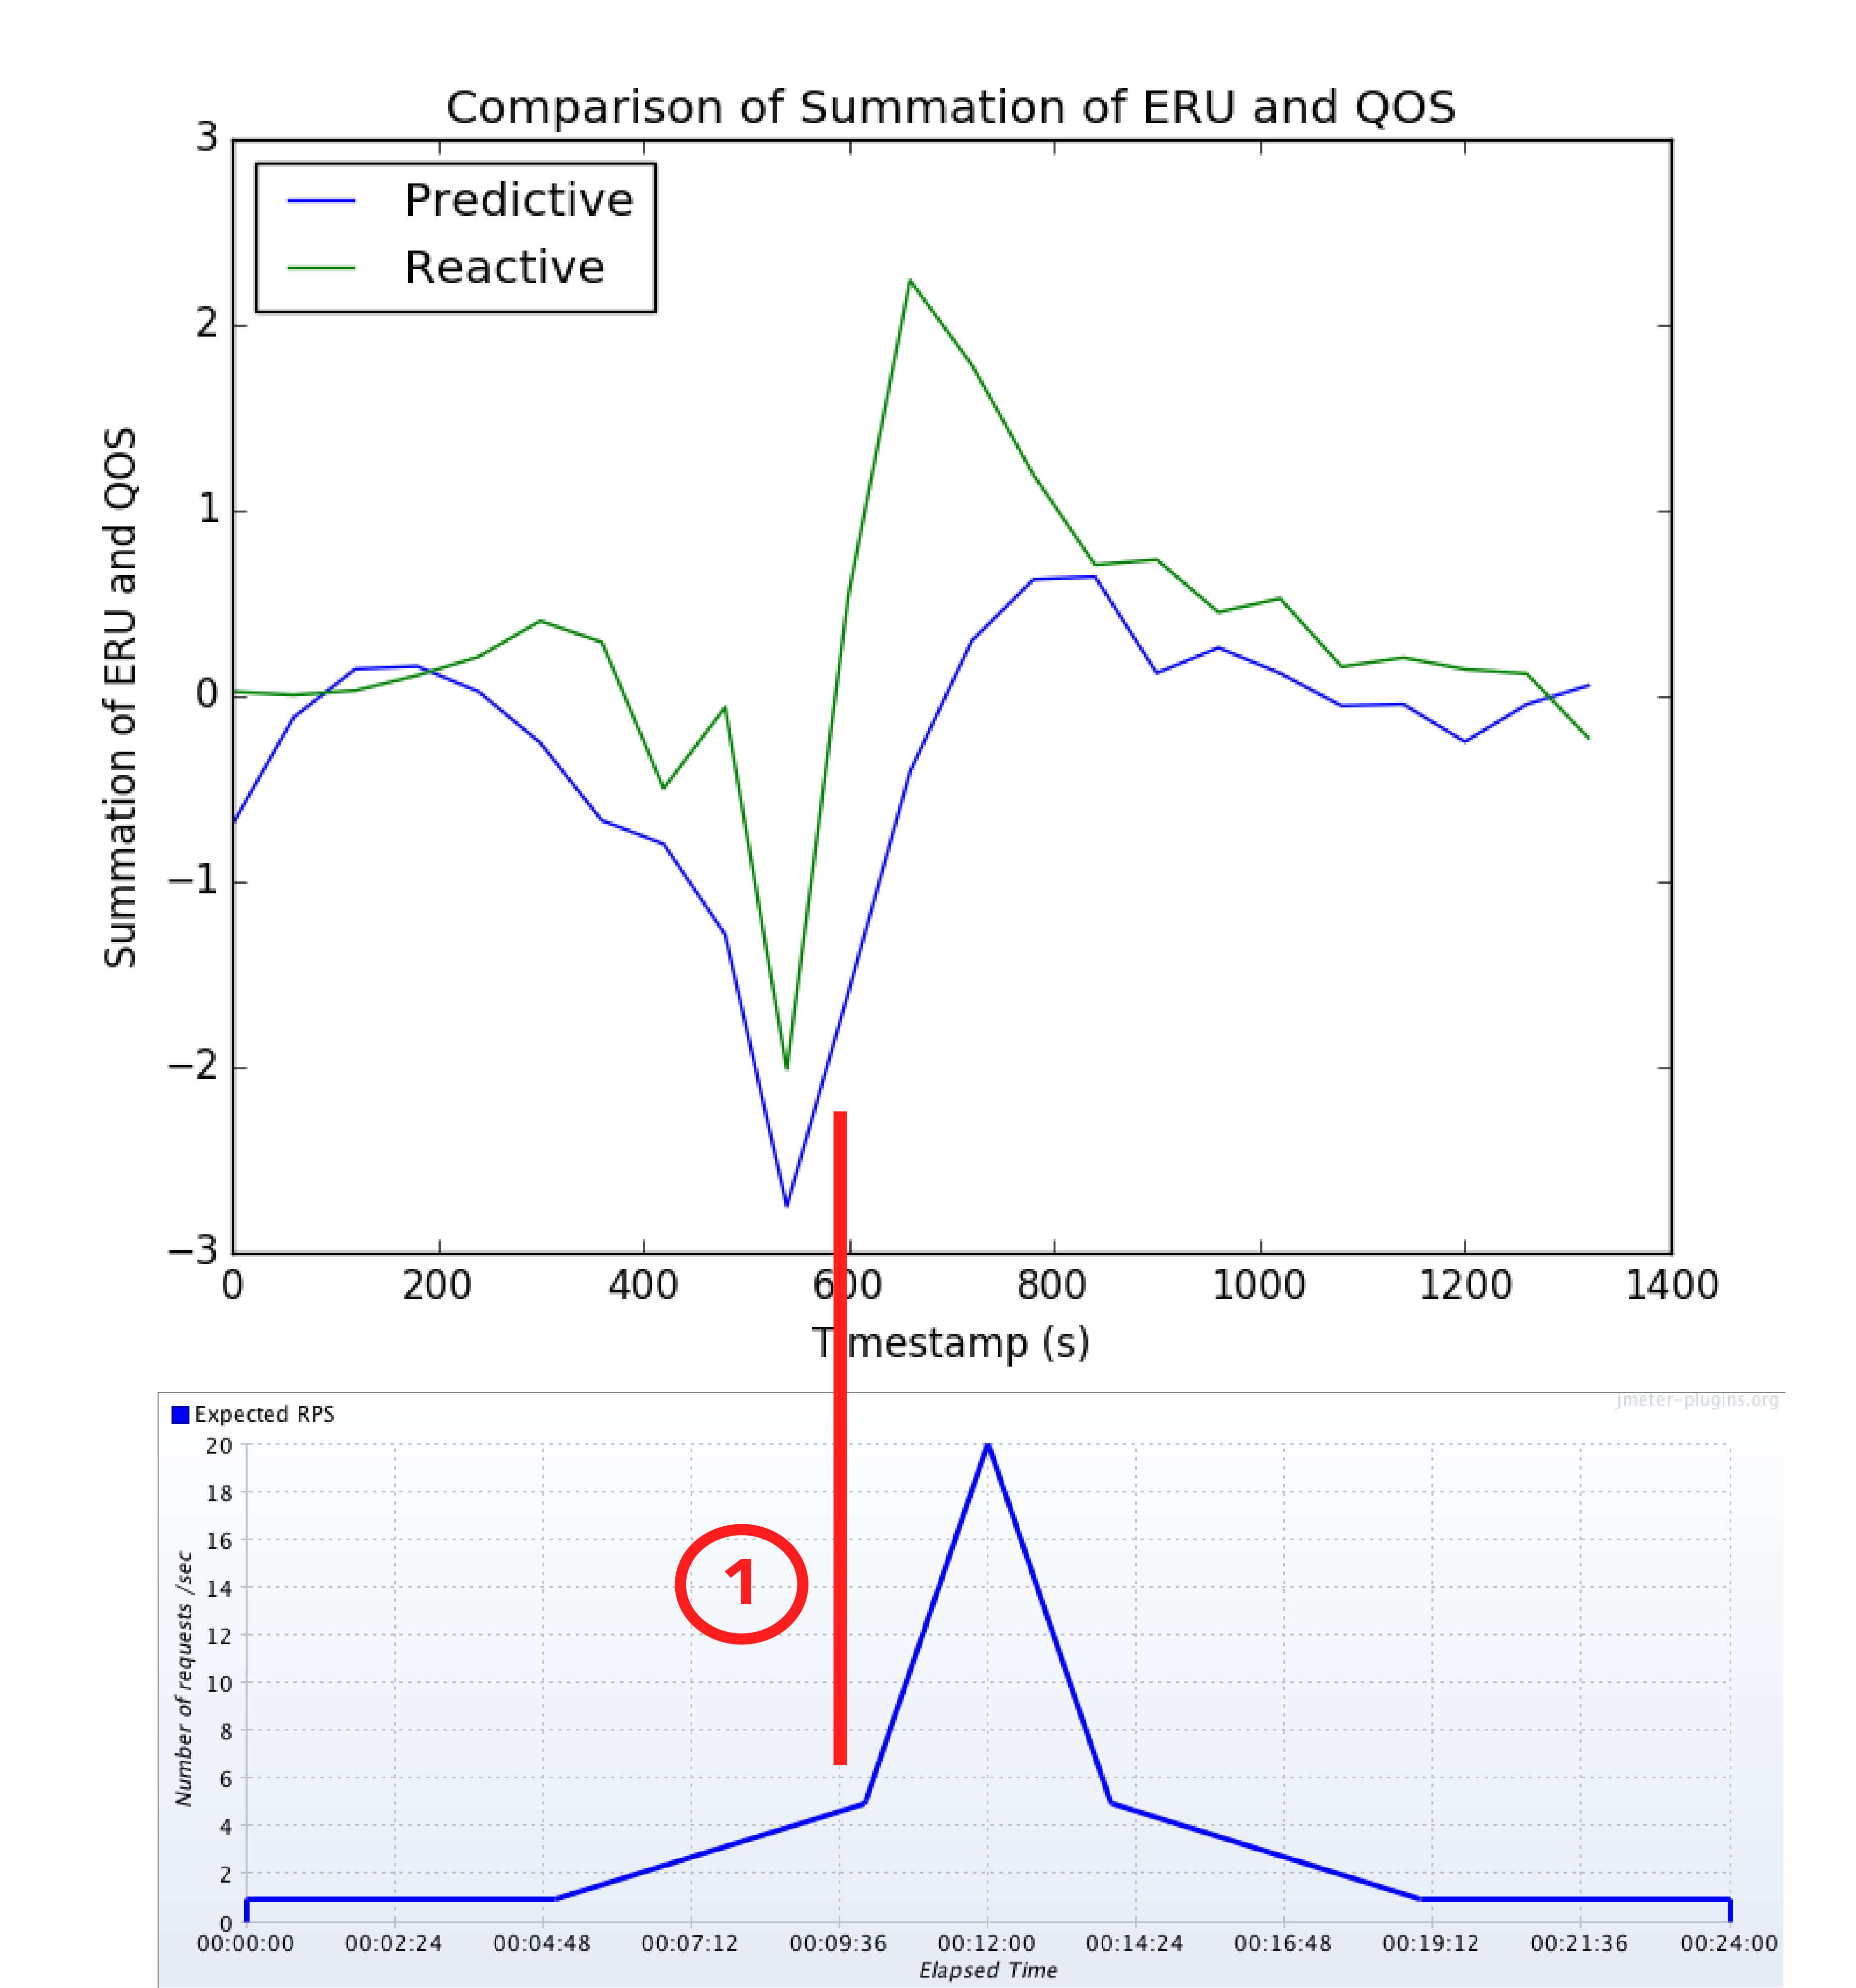
\includegraphics[scale=.70]{flash-crowd-short-labelled.png}}
  \caption{A comparison of the summation of ERU and QoS for
    predictive and reactive auto-scaling for 135s, flash-crowd.}
  \label{fig:135s-flash-crowd-labelled}
\end{figure}

Figure \ref{fig:135s-flash-crowd-labelled} contains a graph
showing predictive and reactive auto-scaling's different
summations of efficient resource utilization and quality of service over the
course of the \textit{flash-crowd} trial. Again,
we find that predictive auto-scaling is not particularly
beneficial in this context. Specifically, if we look at the moment labelled
$1$ on Figure \ref{fig:135s-flash-crowd-labelled}, we see another instance in which
predictive auto-scaling suffers a severe performance decrease because of
under-provisioning. Because this traffic pattern occurs over such a short
interval, the predictive auto-scaling algorithm is unable to fully recognize and
respond to the flash crowd, and is instead hampered by previous measurements
with a significantly lesser slope. Our line-of-best-fit for prediction has too
small a slope, and thus predictive auto-scaling functions worse than reactive
auto-scaling.

\begin{table}[htbp]
  \centering
  \caption{Difference in Predictive and Reactive Auto-scaling for 135s,
  flash-crowd.}
  \label{tab:135s-flash-crowd}
\begin{tabular}{l c}\hline\hline
    \multicolumn{1}{c}{\textbf{Measure}} & \textbf{Value} \\ \hline
     p-value & 0.802 \\
     z-score & -.850 \\
     std\_dev & 0.695 \\
     mean & -0.591
  \end{tabular}
\end{table}

Figure \ref{fig:135s-flash-crowd-labelled} shows that predictive
auto-scaling is fairly detrimental on the \textit{flash-crowd} traffic pattern.
Given Table \ref{tab:135s-flash-crowd}, we are still not able to claim
statistical significance with respect to these results, but we should be fairly
confident that this current iteration of predictive auto-scaling is not an advisable addition
when expecting flash crowds.

